\vspace{-2pt}
\section{Methodology \& Dataset}
\vspace{-4pt}

Our study focuses on the cellular network deployment of a top-tier MNO in a Western European country with over 40 million connected devices. 
During February - March 2023, the MNO tested five different energy efficiency strategies for the RAN, each one over a week, using commercial solutions from equipment vendors (see Table~\ref{tab:mno-trials}).
We focus here on strategies that rely on cell sleep energy efficiency policies, where specific cells within base stations are put into a lower-power sleep mode during times of low traffic load.
%\ael{Orlando, add here a very short definition of what this policy actually does, even if you do explain this later in the following section}

We collect fine-grained KPIs at the cell level, and leverage this data to evaluate the different strategies in terms of the trade-off between estimated energy savings and the impact on end-user performance.

% \begin{table}[!t]
%     \caption{\small Energy saving strategies tested by the MNO.\jo{if you have space, put the text in this table bigger, ideally the same size you have for table 2}} 
%     %\om{Highlight and be clear that ON mean that the energy-saving policy is active, not that the capacity booster is ON}
%     \label{tab:mno-trials}
%     \resizebox{1.0\columnwidth}{!}{%
%     \centering
%     \begin{tabular}{l c c c c}
%     &  & & \multicolumn{2}{c}{\textbf{Load Thresholds}} \\
%     \cline{4-5}
%         \textbf{Strategy} & \textbf{Trial period} & \textbf{Deployment time window} & \textbf{Policy ON} & \textbf{Policy OFF} \\
%         \hline
%          Night-loose & Week 1 & 23h - 6h (night) & 5\% & 10\% \\
%          Night-strict & Week 2 & 23h - 6h (night) & 10\% & 20\% \\
%          Full-loose & Week 3 & 24h (all day) & 5\%  & 10\% \\ 
%          Full-moderate & Week 4 & 24h (all day) & 7\%  & 12\% \\ 
%          Full-strict & Week 5 & 24h (all day) & 10\%  & 15\% \\ 
%     \end{tabular}
%     }
%     %\vspace{-6mm}
% \end{table}

\begin{table}[!t]
    \caption{\small Energy saving strategies tested by the MNO.
    % \jo{if you have space, put the text in this table bigger, ideally the same size you have for table 2}
    } 
    %\om{Highlight and be clear that ON mean that the energy-saving policy is active, not that the capacity booster is ON}
    \label{tab:mno-trials}
    \resizebox{1.0\columnwidth}{!}{%
    \centering
    \begin{tabular}{l c c c}
    & & \multicolumn{2}{c}{\textbf{Load Thresholds}} \\
    \cline{3-4}
        \textbf{Strategy} & \textbf{Deployment time window} & \textbf{Policy ON} & \textbf{Policy OFF} \\
        \hline
         Night-loose & 23h - 6h (night) & 5\% & 10\% \\
         Night-strict & 23h - 6h (night) & 10\% & 20\% \\
         Full-loose  & 24h (all day) & 5\%  & 10\% \\ 
         Full-moderate  & 24h (all day) & 7\%  & 12\% \\ 
         Full-strict & 24h (all day) & 10\%  & 15\% \\ 
    \end{tabular}
    }
    \vspace{-4mm}
\end{table}


\begin{figure}[!t]
    \centering
    \subfloat{
\includegraphics[width=.9\columnwidth]{images/frequencies_dynamic/cell_sleep_dynamic_legend.pdf}}
    \setcounter{subfigure}{0}
    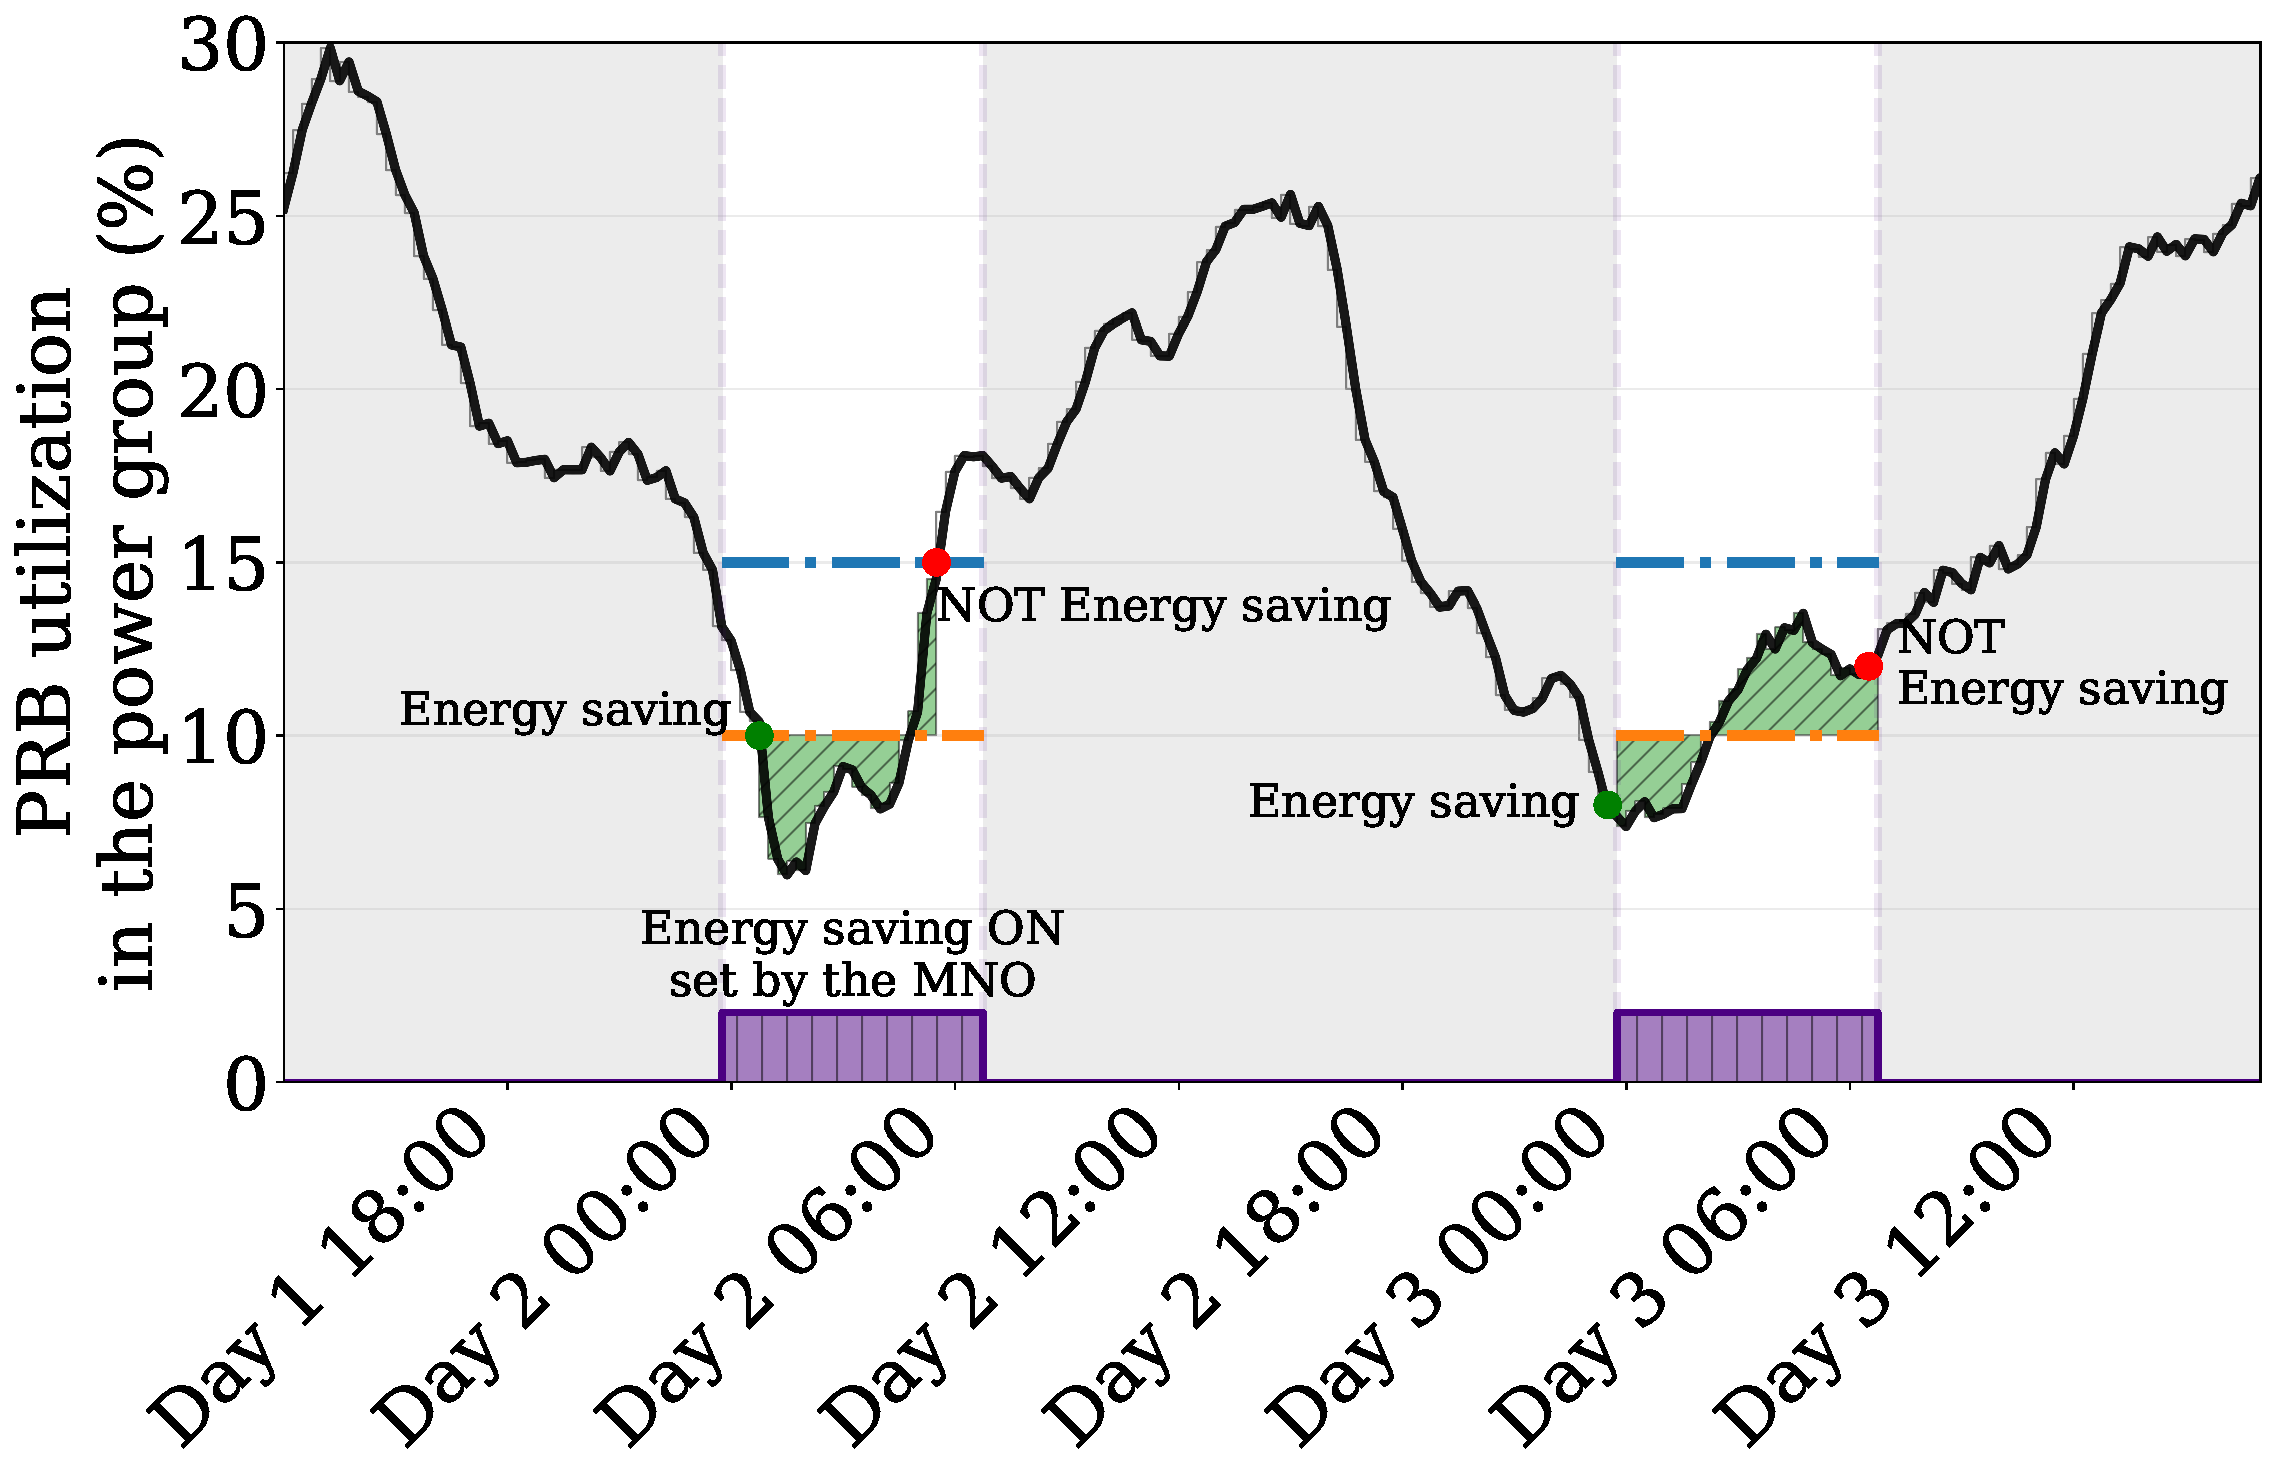
\includegraphics[width=0.95\columnwidth]{images/frequencies_dynamic/cell_sleep_dynamic.pdf}
    \vspace{-4pt}
    \caption{\small Example of energy saving strategy. During the policy deployment time window (purple intervals on the x-axis), a PRB utilization (on the y-axis) dropping below the Policy ON threshold puts the cell in sleep mode. A PRB utilization rising above the Policy OFF threshold wakes the cell from sleep mode. The strategy is disabled outside the policy deployment time window.
    % \js{include the configurable parameters: Active Time Interval, on/off thresholds, Time To Trigger; Y label "PRB utilization (\%)"; X label: don't say "hours". It seems the sample period is too long.}.
    % \mf{\emph{right next to Table~\ref{tab:mno-trials}}, so that it is clear what the values in that table refer to}
    % \js{For the second event, draw a dashed vertical line from the limits of the active time interval to the intersection with the PRB utilization curve; and maybe label it as "NOT Energy saving <br> (end of policy time window)"}
    \label{fig:energy_saving_behaviour}
    }
    \vspace{-15pt}
\end{figure}

\subsection{RAN energy saving strategies}
\label{subsec:background-energy-saving}
\vspace{-2pt}

Figure~\ref{fig:energy_saving_behaviour} illustrates the general behavior of the commercial energy saving solutions tested by the MNO. 
All solutions rely on continuous monitoring of the Physical Resource Block (PRB) utilization, \ie the portion of fundamental radio resource units available in a cell that are allocated to users for data transmission or reception.
PRB utilization is tracked at the level of each \textit{power group}, \ie the set of all cells covering a same geographical area over different frequency bands.
%; the power group is characterized by a predefined order in which its cells should be switched ON/OFF.

The tested solutions apply dynamic cell sleeping strategies based on the time evolution of the average PRB utilization in cells of a power group. 
With reference to Figure~\ref{fig:energy_saving_behaviour}, the following parameters define an energy efficiency strategy.


\textbf{Policy deployment time window:} the time period in which the energy saving policy is enabled. In the strategies that we analyze (Table~\ref{tab:mno-trials}), \textit{Night-loose} and \textit{Night-strict} are active during night time, \ie the deployment time window spans 23:00 to 06:00. The other policies operate all day.

%To this end, the energy saving solution uses a proprietary formula that produces a load estimate at the power-group level, which combines a weighted sum of the PRB utilization of cells depending on their frequency bands. \js{would you keep the previous sentence?} 
\textbf{ON/OFF load thresholds:} These thresholds set the PRB utilization levels that trigger the activation (ON) or deactivation (OFF) of energy-saving policies. When the average PRB utilization in a power group falls below the ON threshold, the energy efficiency solution identifies the cell to send in sleep mode.%
\footnote{Due to non-disclosure agreements with the MNO, we cannot detail the strategy adopted by the tested solutions to select the cell put to sleep.}
%assuming users on these cells will move to others within the same power group (which is far from the reality as discussed later in Section~\ref{sec:evaluation-energy_savings}).
%This strategy aims to maintain PRB utilization of active cells in the power group
% \jo{how many active cells? neighbour active cells? surrounding active cells?} 
%below the OFF threshold.
Conversely, if PRB utilization exceeds the OFF threshold and cells in the power group are in sleep mode, then one of the sleeping cells is woken up. In the MNO trials (Table~\ref{tab:mno-trials}), each strategy sets different ON/OFF load thresholds that represent various levels of aggressiveness: higher thresholds entail higher energy saving, while they may impact more the end-user performance. This characterization of such a trade-off is part of the focus of our study.
%further analyzed in Section~\ref{sec:evaluation-energy_savings}.

\textbf{Time to trigger:} refers to the delay between exceeding the ON/OFF load thresholds and the activation or deactivation of the energy-saving mechanism, designed to prevent erratic switching due to rapid load fluctuations. In our case, the MNO has set this delay to 10 minutes for the cell sleep process and 5 minutes for reactivation. To minimize user impact, the cell power is gradually reduced before a full shutdown, ensuring a smooth transition for users from the cell edge to its center.
All tested solutions adopt the same time to trigger implementation.
%This makes the coverage area to be gradually reduced and guarantees a smooth transition of UEs from the edge to the center of the cell. Likewise, the solution applies a contention mechanism that prevents switching off cells in case there are ongoing emergency calls or queued messages for Earthquake and Tsunami Warning System (ETWS) or Commercial Mobile Alert System (CMAS), thus keeping the network at full capacity under emergency events.


\begin{figure}[!t]
    \centering
    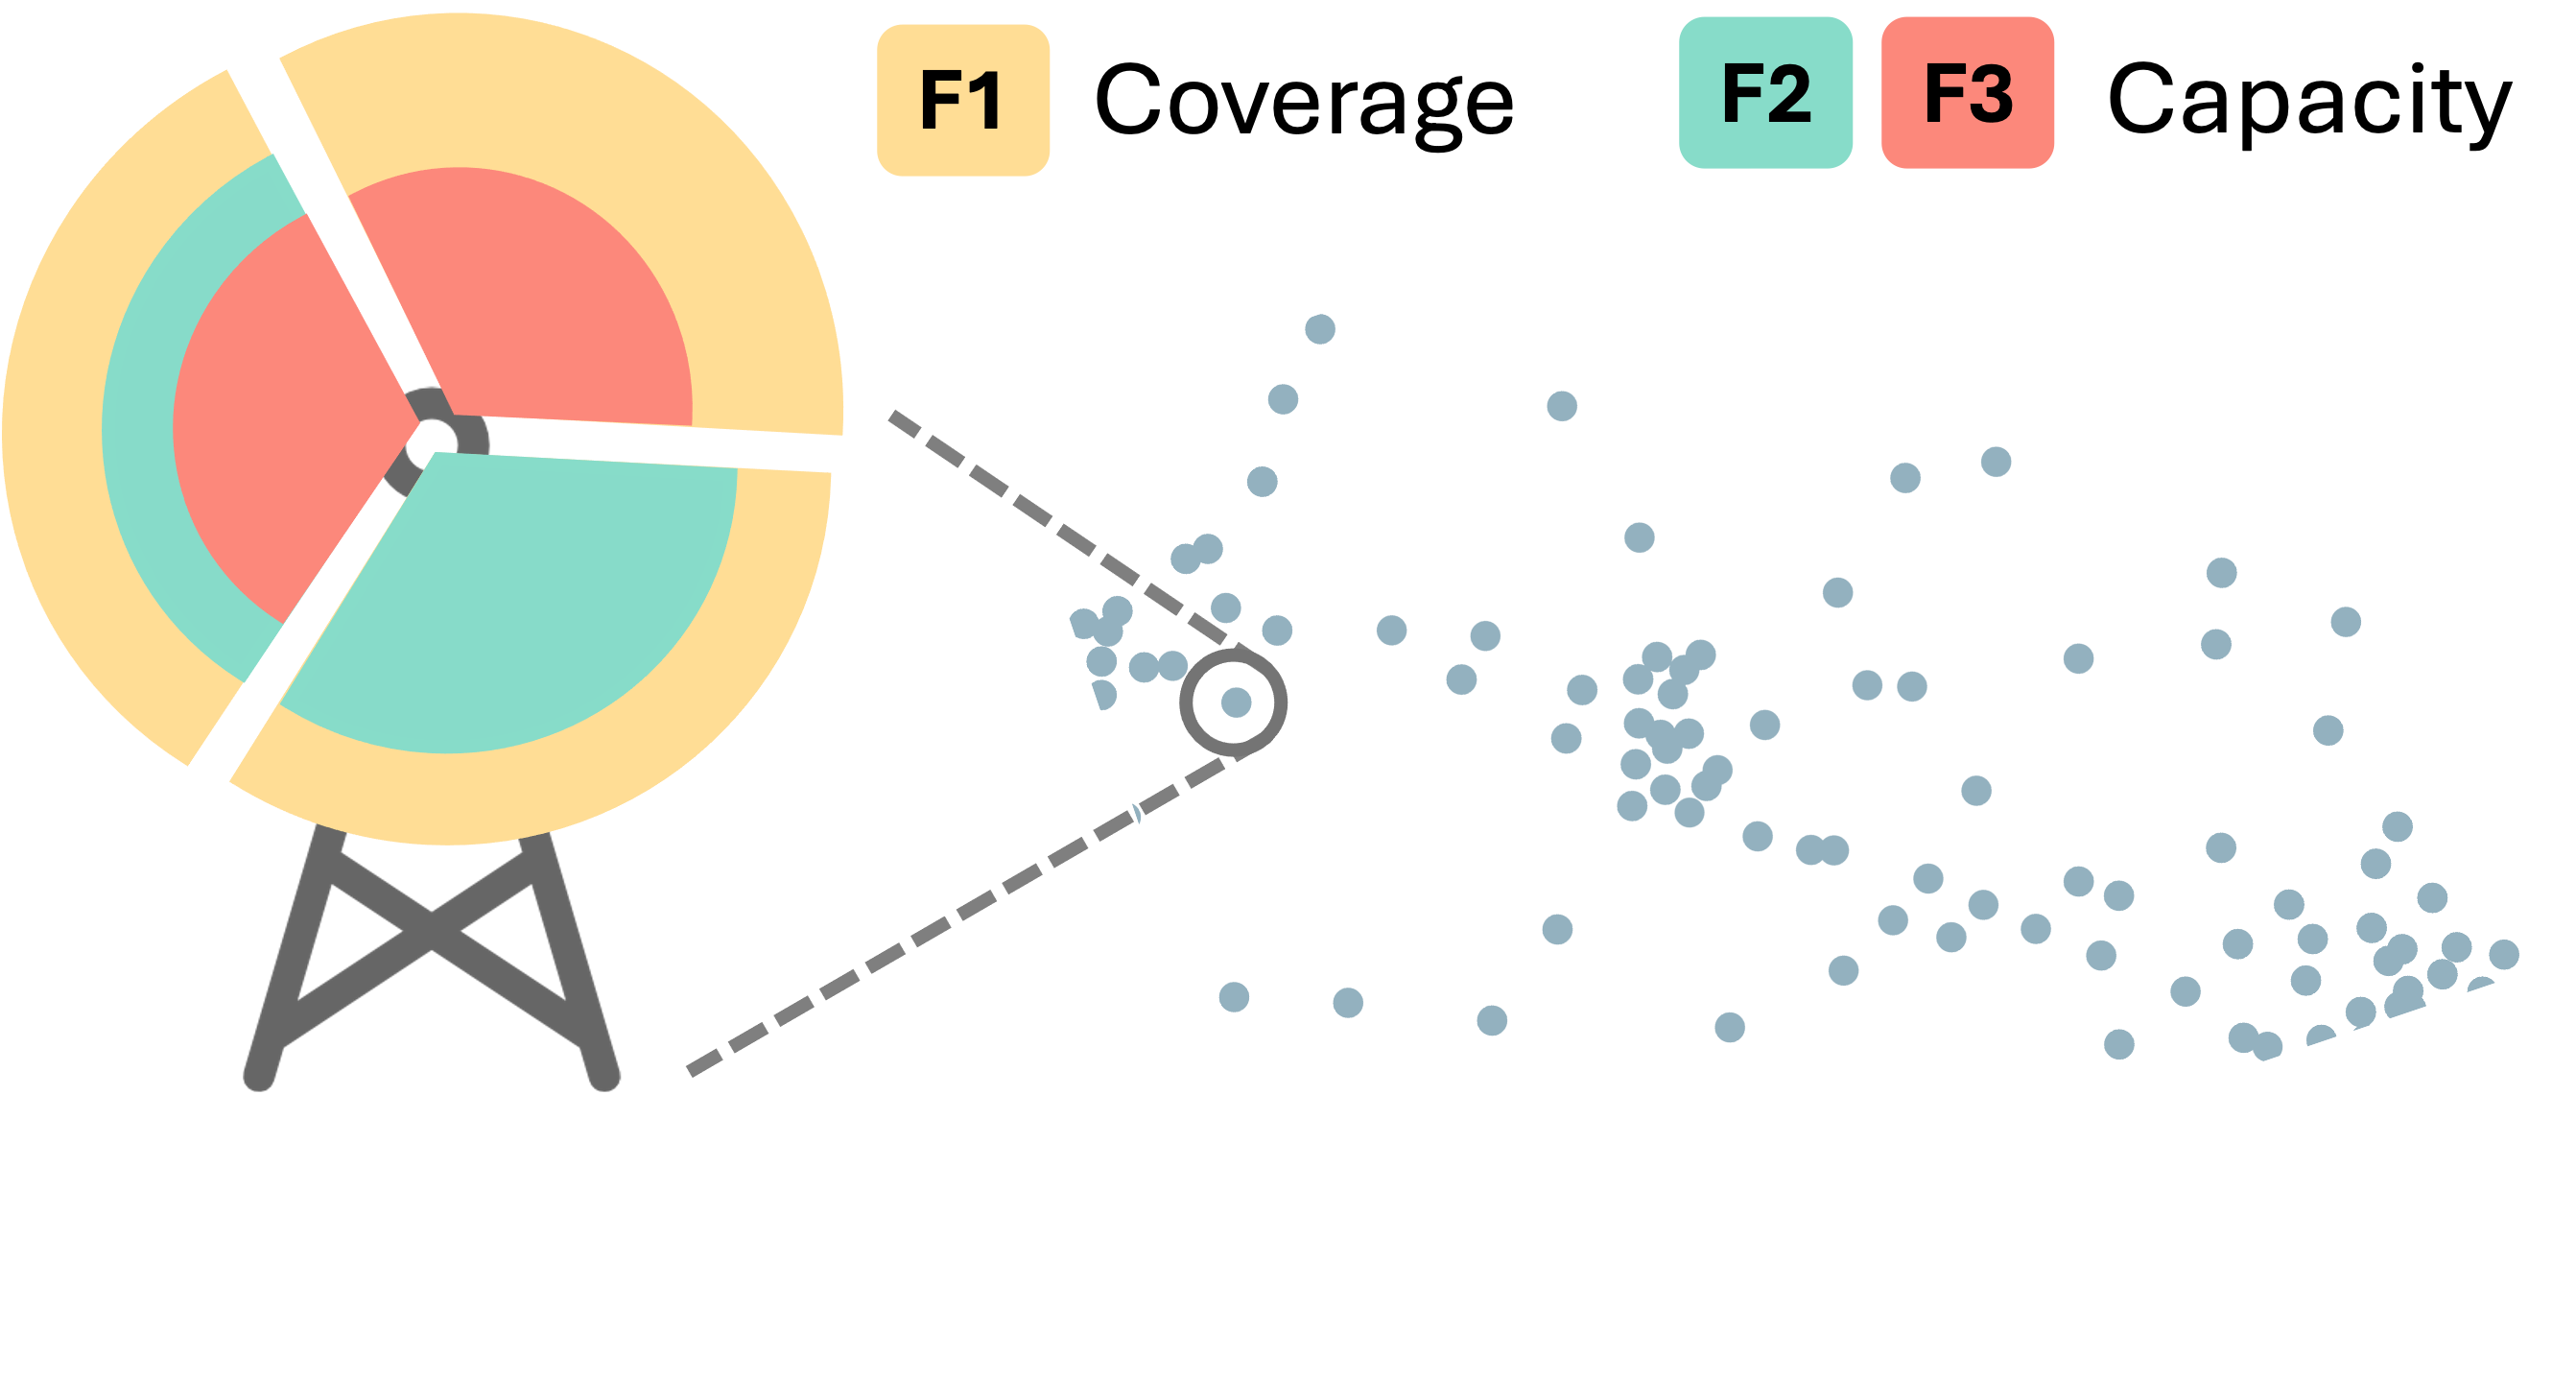
\includegraphics[width=.85\columnwidth,,trim={0 50pt 0 0},clip]{images/frequencies_dynamic/antenna_frequencies.png}
    \vspace{-4pt}
    \caption{\small Example of a three-sector site with cells deployed on three different frequency bands, for coverage and capacity. Blue dots represent base stations included in a specific trial. 
    \label{fig:capacity_booster_frequencies}
    }
    \vspace{-15pt}
    % \js{Display area as a circle and slightly randomized locations}\js{coverage in gray and the rest in the same colors? Also, differentiate capacity and coverage groups in the legend}
\end{figure}


\subsection{Energy saving trials}\label{subsec:energy-saving-trials}
\vspace{-2pt}

In line with standard deployment strategies, the MNO catalogs its licensed frequency bands into two classes: low-frequency bands that are used to optimize \textit{coverage}, and mid- to high-frequency bands that are dedicated to enhancing \textit{capacity}. From these, capacity cells are the only ones that implement energy saving policies, while coverage cells typically remain untouched to guarantee service availability over the entire geography. Accordingly, each power group comprises a set of capacity cells and one or more coverage cells. %, which should %$(i)$ provide service to the UEs of the capacity cell, should this one shut down, and $(ii)$ assist the capacity antennas to start the wake up process. Thus, 
%which assist capacity cells to start the wake-up process when the load exceeds the OFF threshold.
Figure~\ref{fig:capacity_booster_frequencies} shows an example of a cell site located in one of the regions the MNO used for the pilot. A three-sectored site uses cells operating in three frequency bands. Cells in the F1 band are used for coverage, while F2 and F3 bands are used for capacity and are dynamically 
put to sleep mode and woken up as dictated by the deployed energy saving strategy. % (see Sec.~\ref{subsec:background-energy-saving}).

The MNO performed trials of five energy saving strategies, each over a one-week period (see Table~\ref{tab:mno-trials}), and over two geographic regions delimited by specific Tracking Area Codes (TAC). Table~\ref{tab:regions} summarizes the RAN infrastructure features in two trial regions, which include diverse population and cell deployment densities (cells/sq. km.). Hereafter, we refer to these regions as \textit{Dense} and \textit{Sparse}, respectively. 
Energy saving strategies were only tested on LTE cells, which account for $71.51\%$ and $54.14\%$ of the cells deployed in the two regions, and all other RATs, including 2G, 3G and 5G, were excluded from the trial. Capacity cells, which are affected by the energy saving policy, account for $23.05\%$ of the tested cells in Dense regions and $27.43\%$ in Sparse regions.

% \js{Remove this paragraph ?} Note that the definition of power groups (\ie coverage and capacity cells under the same energy saving domain) is a delicate process that may have some impact on the final energy savings. Nevertheless, the aforementioned trials consider predefined power groups and focus on evaluating the impact of the five energy saving strategies (Table~\ref{tab:mno-trials}) across the two geographical trial regions (Table~\ref{tab:regions}).

\vspace{-2pt}
\subsection{Measurement data feeds}\label{data-feeds}
\vspace{-2pt}

\begin{table*}[!t]
\centering
\caption{\small Description of the regions under study
\label{tab:regions}}
\begin{tabular}{lcccccc}
\toprule
\textbf{Region name} & \textbf{Area $km^2$} & \textbf{LTE share} & \textbf{LTE Density (cells/sq. km.)} & \textbf{LTE cells / site} & \textbf{Capacity cells (\%)}\\

\midrule
Dense region & 189.28 & 71.51\% & 5.41 & $11.0 \pm 6.10$ & 23.05\% \\
Sparse region & 4986.82 & 54.14\% & 0.21 & $8.5 \pm 5.98$ & 27.43\% \\
\bottomrule
\end{tabular}
\vspace{-4mm}

\end{table*}

For our evaluation, we use cell-level measurements from LTE cells in the two study regions (Table~\ref{tab:regions}), collected throughout the whole trial period. Below, we describe the data feeds that were processed and combined for our analysis.
%Also, as a reference for our evaluation, we collect measurements on the same regions two weeks before the trials (Feb 8-Feb 15, 2023)\om{Right!, but we are not showing any results about this; it is still nice to comment about it, can you phrase in a way that expresses that we check it and didn't find major different beyond the trials and the network activity was ok/normal, and also in other areas}. For this, we rely on two main data feeds that the MNO injects into its BigData measurement platform: 

\textbf{Radio access network deployment}:
We collect an inventory of all the cells deployed in the two regions of study. This includes cell-level information such as the location (lat/lon coordinates), the eNodeB ID, the orientation (azimuth), tilt, antenna manufacturer and model, and the carrier (\ie frequency channels). This inventory is updated daily to reflect changes in the network topology, such as the deployment of new cells and the decommissioning of older technologies.

\textbf{Radio access network KPIs}:
The MNO monitoring infrastructure collects more than 160 KPIs at the cell-level for all the RATs deployed, including from GSM (2G) to the newest 5G NR cells. Measurements are collected every 15 minutes and averaged over hourly intervals. %, which are eventually stored in a BigData cluster for long retention periods. 
In our study, we evaluate the different energy-saving strategies using three main KPIs: (i) \textit{cell availability}, which measures the amount of time a cell was woken up within a specific hour, with granularity down to seconds; (ii) \textit{cell load}, expressed as the PRB utilization in downlink%
\footnote{As most frequency bands use FDD, downlink channels get congested earlier than uplink ones, hence downlink PRB utilization is a better indicator.};
and (iii) \textit{average user throughput}, which indicates the average data rate served by the cell.

\textbf{Mobility management signaling}:
We collect control-plane signaling messages from the Mobility Management Entity (MME) of the 4G Evolved Packet Core (EPC). This data captures all mobility-related events (e.g., attach, detach, handover) at the LTE cells involved in the MNO trials, with timestamps recorded to the millisecond. We use this data %in Sec.~\ref{sec:evaluation-energy_savings}
to analyze user transitions during cell sleep or wake up events and identify the \textit{fallback cells}, \ie the cells that absorb the load and UEs.
% within each power group.